% Chapter Template

\chapter{A Comparison of the NREL 5-MW Wake Characteristics Using Both SOWFA and OVERFLOW2} % Main chapter title

\label{Chapter5} % Change X to a consecutive number; for referencing this chapter elsewhere, use \ref{ChapterX}


%----------------------------------------------------------------------------------------
%	SECTION 1
%----------------------------------------------------------------------------------------

\section{Introduction}\label{section5-1}
Utility scale wind power is often installed as wind farms, with several turbines installed in close proximity to each other. Many established simulation tools used in the wind industry simulate single turbines\cite{jonkman2005,chow2012,chow2013,platt2012}. While single turbine simulation tools are valuable, they fail to capture the turbine-to-turbine interactions that are common in a wind farm. The National Renewable Energy Laboratory's (NREL) Simulator fOr Wind Farm Applications (SOWFA) is a wind farm simulation tool.\cite{churchfield2012} SOWFA uses a large eddy simulation (LES) methodology to model a flow field, while using a computationally inexpensive but well established aero-elastic simulation to model turbines in the flow field. By coupling a high fidelity flow field model to a medium fidelity turbine model SOWFA hopes to accurately model wind farm aerodynamics without incurring the high computational cost of modeling a turbine with CFD techniques. SOWFA has the potential to be a valuable tool for studying wind farm phenomena such as turbine-to-turbine wake interactions\cite{lee2012}, plant level controls\cite{fleming2013}, and complex terrain\cite{churchfield2013}. However, SOWFA is still a relatively new simulation tool and more validation of SOWFA's capabilities would be beneficial. This chapter will attempt to directly compare the predicted NREL 5-MW wake structure and behavior using both SOWFA and a Reynolds-averaged Navier-Stokes (RANS) method, OVERFLOW2. The NREL 5-MW rotor is analyzed at several wind speeds and the aerodynamic performance predicted by SOWFA and OVERFLOW2 are compared. This chapter will also examine how SOWFA results are affected by downstream length and grid resolution of the near-wake grid.

The study documented in this chapter was carried out in collaboration with Dr Raymond Chow.  Dr Chow performed the RANS simulations discussed below and provided several of the figures, as noted in the figure captions. Dr Chow also featured these RANS simulations in a pair of publications.\cite{chow2012,chow2013}

%----------------------------------------------------------------------------------------
%	SECTION 2
%----------------------------------------------------------------------------------------

\section{Hybrid LES Method}\label{section5-2}

%-----------------------------------
%	SUBSECTION 2-1
%-----------------------------------
\subsection{SOWFA}\label{section5-2-1}
In SOWFA, the flow field is modeled using a large eddy simulation (LES) methodology based on the open source CFD software openFOAM \cite{churchfield2012}. The large-eddy simulation is governed by the momentum transport equation, with terms accounting for convection and the the Coriolis force, shown in Equation \ref{eq1} and the potential temperature transport equation shown in Equation \ref{eq2}. The last term in Equation \ref{eq1} ($f_{i}^{T}$) accounts for other forces applied to the flow field (from the wind turbine actuator line model). Sub filter scale momentum and temperature fluxes are calculated using the Smagorinski model \cite{smagorinsky1963}. The filter length scale is defined as $\Delta =(\Delta x\Delta y\Delta z)^{1/3}$ where $\Delta x$, $\Delta y$, and $\Delta z$ are the local cell lengths. 
\begin{equation}
\frac{\partial \bar{u}_{i}}{\partial t} +\frac{\partial }{\partial x_{i}}(\bar{u}_{i}\bar{u}_{j})=-2\epsilon _{i3k}\Omega _{3}\bar{u}_{k}-\frac{\partial \bar{p}}{\partial x_{i}}-\frac{1}{\rho_0}\frac{\partial }{\partial x_j}\bar{p}_0(x,y)-\frac{\partial }{\partial x_j}(\tau_{ij}^{D} )-g\left( \frac{\bar{\theta }-\theta_0}{\theta_o}\right)\delta _{i3}+\frac{1}{\rho _0}f_{i}^{T}
 \label{eq1}
\end{equation}  

\begin{equation}
\frac{\partial \bar{\theta}}{\partial t}+\frac{\partial }{\partial x_j}(\bar{u}_j\bar\theta)=-\frac{\partial }{\partial x_j}(q_j)
 \label{eq2}
\end{equation}  



%-----------------------------------
%	SUBSECTION 2-2
%-----------------------------------
\subsection{Actuator Line Model}\label{section5-2-2}
The LES model is 2-way-coupled to the aeroelastic turbine model using actuator line models of the turbine blades\cite{shen2002}. Because of the high Reynolds number flow over the viscous surface of the rotor, it is currently difficult to model the geometry of the rotor accurately directly with an LES method. As such a different method to model the rotor flow is needed if the advantages of LES are to be gained in the global domain. Previous methods have utilized actuator disk models within LES domains, but the resultant flow fields do not capture the vortical wake structure of a rotor flow field. Instead, due to the averaging of the loading across the entire rotor plane, only a smeared out momentum deficit is captured in the wake\cite{mirocha2014}. SOWFA attempts to improve on this by using an actuator line method. Within the LES domain, the rotating blades are modeled using unsteady, rotating line elements. Along each element, the local LES flow characteristic is determined and transferred to FAST at each coupled time-step. The local blade loading is determined in FAST and the reaction forces are returned to the LES solver and perturbs the local flow field.

This of course greatly simplifies the aerodynamic modeling for the rotor itself, but the approximate rotor loading and corresponding flow field impact should be correctly captured. Furthermore, using the rotating actuator line method should also lead to an unsteady, rotating wake structure that more closely resembles an actual rotor flow. This improved wake structure, with discrete tip and root vortices, could lead to improved predictions in terms of wake coherence, wake-turbine interaction, and atmospheric boundary layer impact.



%-----------------------------------
%	SUBSECTION 2-3
%-----------------------------------
\subsection{Aeroelastic Turbine Model}\label{section5-2-3}
Accurately modeling a wind turbine with an aeroelastic code is far less computationally expensive than modeling a wind turbine with traditional CFD methods such as viscous 3-D RANS. In SOWFA wind turbines are modeled using a version of NREL's FAST that has been coupled with SOWFA. FAST is a medium fidelity aeroelastic wind turbine modeling tool.  It is widely used in the wind industry for turbine design. FAST models turbine structural dynamics as a combination of modal dynamics and multibody dynamics. The multibody dynamics are calculated using Kanes' method\cite{jonkman2013}.  FAST models aerodynamic loading on the turbine using blade element-momentum (BEM) theory. In BEM theory turbine blades are treated as  a collection of discrete 2-D airfoil segments that move in space as the turbines blades rotate and flex. The aerodynamic forces on each airfoil segment are determined from the local air flow field, as well as the motion, orientation, and aerodynamic properties of the airfoil.  The aerodynamic forces on the rotor are determined by summing the forces on all of the blade segments and applying a series of correction factors to account for phenomenon such as tip and root vortices, and dynamic stall\cite{burton2011}. 


%-----------------------------------
%	SUBSECTION 2-4
%-----------------------------------
\subsection{LES Computational Domain}\label{section5-2-4}
The computational domain extends 20\emph{R} upstream, where the NREL 5-MW rotor radius \emph{R} is equal to 63 m, and 40\emph{R} downstream of the rotor. In the rotor plane the computational domain extends 20\emph{R} from the center of the rotor in both the vertical and horizontal directions. Initially this rectangular domain is composed of 32 m $\times$ 32 m $\times$ 32 m cells, but portions of the domain go through a series of grid refinements to reduce the size of the cells near the NREL 5-MW rotor and wake. The refinement regions are a series of 5 concentric cylinders with centerlines laying on the rotational axis of the NREL 5-MW rotor and having the dimensions shown in Table \ref{Table5-1}. Table \ref{Table5-1} describes the refinement regions in both meters and in terms of the NREL 5-MW rotor radius \emph{R}. This grid refinement scheme is modified for some of the simulations in sections \ref{section5-4-2} and \ref{section5-4-2}. The modifications are described in those sections.  SOWFA has the capability to model ground effects, as well as the effects of neutral and unstable atmospheric conditions. However, in order to match the OVERFLOW2 simulations, those capabilities are not used and this study is limited to a rotor in a uniform and unbounded freestream.

\begin{table}
\centering
\begin{tabular}{c c c c c}
\hline
Refinement & Upstream  & Downstream & Radial & Max Cell Size\\
Region & (\emph{R}) & (\emph{R})  &  (\emph{R}) & in Region\\
\hline
1 & 8.5\emph{R} (536 m)  & 40\emph{R} (2320 m) & 8.9\emph{R} (561 m)  & 16 m $\times$ 16 m $\times$ 16 m\\
2 & 4.5\emph{R} (284 m   & 40\emph{R} (2320 m) & 4.9\emph{R} (309 m)  & 8 m $\times$ 8 m $\times$ 8 m\\
3 & 2.5\emph{R} (158 m)  & 24\emph{R} (1512 m) & 2.9\emph{R} (183 m)  & 4 m $\times$ 4 m $\times$ 4 m\\
4 & 1.5\emph{R} (95 m)    & 12\emph{R} (756 m)   & 1.9\emph{R} (120 m)  & 2 m $\times$ 2 m $\times$ 2 m\\
5 & 1.0\emph{R} (63 m)    & 6\emph{R} (378 m)     & 1.4\emph{R} (88 m)   & 1 m $\times$ 1 m $\times$ 1 m\\
\hline
\end{tabular}
\caption{ Extents and resolutions of the SOWFA grid refinement regions (distances extending from the center of the rotor).}
\label{Table5-1}
\end{table}


%----------------------------------------------------------------------------------------
%	SECTION 3
%----------------------------------------------------------------------------------------

\section{RANS Computational Method}\label{section5-3}

%-----------------------------------
%	SUBSECTION 3-1
%-----------------------------------
\subsection{OVERFLOW2}\label{section5-3-1}
OVERFLOW2 is a numerical simulation method that solves the compressible Reynolds-averaged Navier-Stokes equations on structured, overset grids \cite{buning2003,nichols2008}. OVERFLOW2 is a very robust and comprehensive code, allowing for the selection from a variety of numerical schemes, turbulence models, boundary conditions, and time advancement schemes \cite{jespersen1997,nichols2006}. The numerical method selected for this portion of the study will be central difference Euler with a Beam-Warming pentadiagonal scheme \cite{beam1979}. The viscous near-body grids will utilize a spatially 2nd-order method, while the Cartesian off-body grids will use a spatially 4th-order accurate method with 6th-order matrix dissipation term. All solid boundaries are treated as viscous walls, and all calculations are performed fully turbulent, with Menter's two-equation Shear Stress Transport (SST) k$-\omega$ model \cite{menter1994} being used exclusively. Only the Euler terms are solved in the off-body grid system in order to reduce excess numerical dissipation. All unsteady calculations are performed second-order in time using dual-time stepping \cite{nichols2005}. To model the rotation of the rotor, the rotational source term formulation of the Navier-Stokes equations will be used, where the Coriolis and centrifugal force terms are added to the governing equations.



%-----------------------------------
%	SUBSECTION 3-2
%-----------------------------------
\subsection{RANS Computational Meshes}\label{section5-3-2}
The Chimera overset structured grid scheme is employed to model the computational flow domain. This approach allows geometrically complex multi-body configurations to be constructed from sets of relatively simple overlapping body-fitted grids \cite{steger1983,chan2009}. The near-body computational grid is generated with Chimera Grid Tools (CGT) 2.0 \cite{chan2002}. The CGT package contains independent grid generation, manipulation, visualization and diagnosis tools that can be run in batch mode under the OVERGRID graphical interface \cite{chan2002b}. Overlapping grid regions in the hub region and with the off-body grids are cut or IBLANKed using Meakin's object X-Ray method \cite{meakin2001}. Domain connectivity is also performed automatically by OVERFLOW2 using a non-conservative interpolation between overlapping grids. All body-fitted grids are generated with a wall spacing of approximately $y^+\cong0.3$  \cite{chan2002c,bardina1997}. Off-body grids were constructed using a series of cubic Cartesian layers or BRICKS \cite{meakin2001b} automatically generated by OVERFLOW2 based on user specified cell size, growth rate, and far-field distance. Layers of off-body BRICKS are built from the near-body, with each additional layer doubling in cell dimension, and having the benefit of a point-matched donor-injection pair at the overset boundaries. This allows for a very efficient and cost effective way of filling the off-body domain. In this work, the far-field distance will be defined as the distance from the rotor center to one of the five freestream imposed boundaries on the upstream and four Cartesian sides of the domain. In the downstream direction, the inflow/outflow boundary is placed twice this far-field distance away from the rotor. 



%-----------------------------------
%	SUBSECTION 3-3
%-----------------------------------
\subsection{RANS NREL 5-MW Rotor Near-body Grid}\label{section5-3-3}
A fully viscous Overset grid system was developed for the NREL 5-MW rotor. The full 3-bladed rotor was modeled without the use of any symmetry or periodic conditions in the global domain. Each of the three \emph{R} = 63 m blades is defined using an identical set of hub, inboard, outboard and tip near-body grids. The surface grids are hyperbolically grown out approximately 10 m (2.13\emph{c$_{max}$}) away from the body with an O-type topology. The near-body grid system utilized a total of 13M grid points. The off-body grid system extends 20\emph{R}  upstream and around the rotor, and 40\emph{R}  in the downstream direction. The rotor itself is surrounded by an initial uniform Cartesian near-wake grid that extends 6\emph{R}  downstream and 0.5\emph{R}  upstream of the rotor with a constant cell size of 1.0 m. Extensive details of the near-body and off-body grid independence studies can be found in previous studies \cite{steger1983,chan2009,chan2002}. Calculations were continued until both integrated power and thrust values deviated by less than 0.1\% and residuals levels remained effectively constant over a period of 30-40 thousand iterations. All steady-state solutions were run between 120-160 thousand iterations. Time-accurate calculations were performed so that at least a two-order of magnitude drop in the L2-residual was achieved for all grids to ensure temporal convergence. This utilized a physical time-step of 1.4 msec (or rotor azimuthal angle increment of 0.1 degrees per step) and required 25 subiterations per global time-step for convergence. The composite overset grid topology for one of the blades from the baseline NREL 5-MW surface grid is shown in Figure \ref{OFGrid} along with the thickness-to-chord ratio distribution over the span of the blade. 

\begin{figure}[htbp]
 \centering
 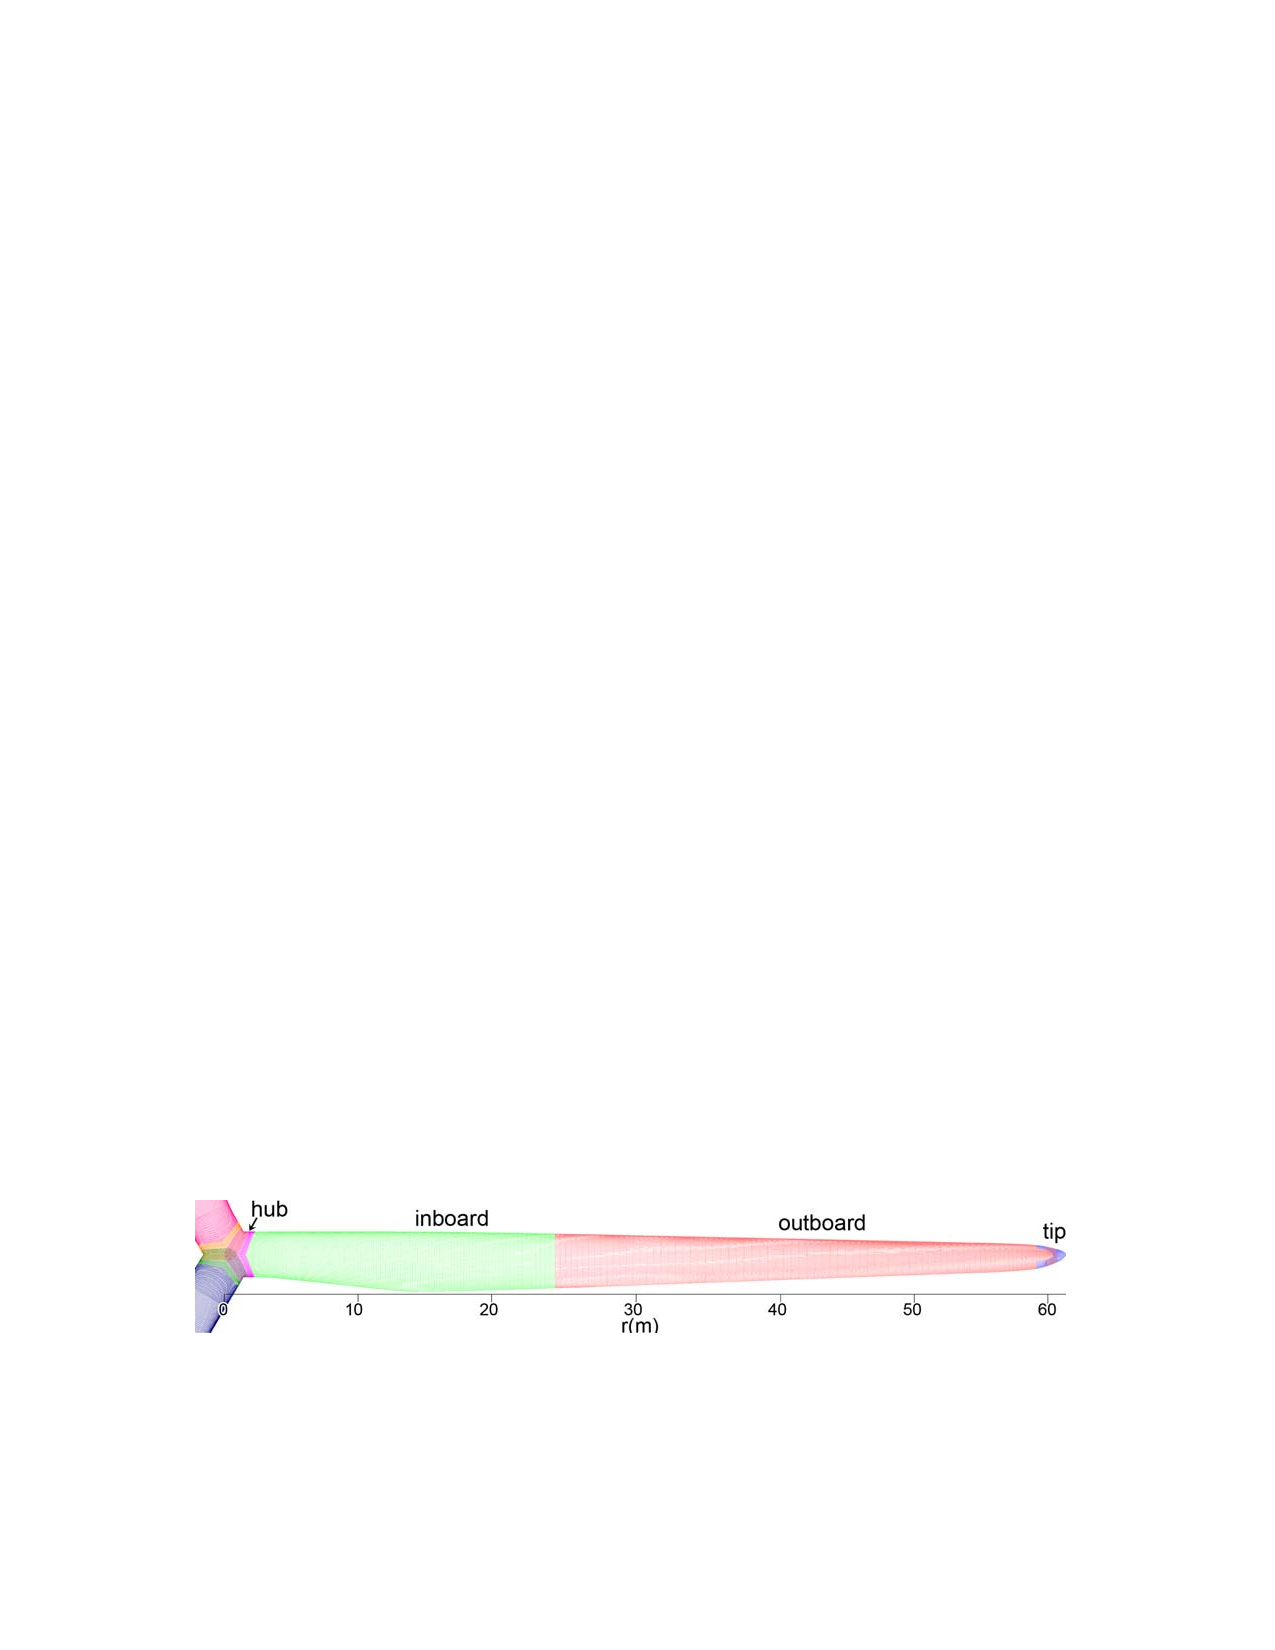
\includegraphics{Figures/ch5Figures/OVERFLOWGrid}
 \caption{ Near-body overset topology of the NREL 5-MW medium resolution grid system. (Source: R. Chow)}
 \label{OFGrid}
\end{figure}   


%----------------------------------------------------------------------------------------
%	SECTION 4
%----------------------------------------------------------------------------------------

\section{Experimental results}\label{section5-4}


%-----------------------------------
%	SUBSECTION 4-1
%-----------------------------------

\subsection{Comparison of SOWFA and OVERFLOW2 Results}\label{section5-4-1}
SOWFA and OVERFLOW2 results are compared for the cases shown in Table \ref{Table2}. The incoming wind speeds (\emph{U$_\infty$}) were chosen to cover three control regions of the NREL 5-MW turbine. In 8 m/s winds the turbine operates in control region 2, variable speed control. In 15 m/s winds the turbine operates in control region 3, variable pitch control. In 11 m/s winds the turbine operates in control region 2.5, the transition between region 2 and region 3. In all cases the incoming wind field is laminar, steady and uniform. The rotor speed and pitch shown in Table \ref{Table2} are the steady state operating conditions of the NREL 5-MW turbine at the corresponding incoming wind speed. Because there are no simulation results for the NREL 5-MW turbine a direct validation was not possible. However, the OVERFLOW2 simulation results were compared to an independent simulation of the NREL 5-MW rotor carried out by S{\o}rensen and Johansen using EllipSys3D\cite{shen2002}. The thrust and power predicted with OVERFLOW2 were found to have good agreement with previous published predictions for the NREL 5-MW\cite{chow2012}.


\begin{table}
\centering
\begin{tabular}{c c c }
\hline
\emph{U$_{\infty}$} & Rotor Speed & Pitch\\
(m/s) & (RPM) & (\degree)\\
\hline
8 & 9.16 & 0\\
11 & 11.89 & 0\\
15 & 12.10 & 10.45\\
\hline
\end{tabular}
\caption{ NREL 5-MW simulation cases}
\label{Table2}
\end{table}

The SOWFA near-wake grid extends 6\emph{R} (378 m) downstream and 1\emph{R} (63 m) upstream, the same dimensions used for OVERFLOW2 simulations. In the radial direction the SOWFA near-wake grid extends 1.4\emph{R} (88 m). This makes the in-plane area of the SOWFA near-wake grid approximately 25\% larger than the 140 $\times$ 140 m OVERFLOW2 grid and provides a constant 25 m spacing between the blade tips and the edge of the near-wake grid. In the rectangular OVERFLOW2 grid the spacing between the blade tips and the edge of the near wake grid varies from 7-36 m depending on the instantaneous orientation of the rotor. Other SOWFA parameters for theses cases are chosen based on best practices\cite{churchfield2012,martinez2012}. The Gaussian projection width was set to the mean chord length of the NREL 5-MW blade  (3.5 m). Each actuator line has 123 elements, ensuring that each actuator element is less than 3/4 the near-wake grid resolution. BEM tip and root losses are disabled because the LES methodology captures the vortical wake. The simulation time step is chosen to be 0.01s so turbine blade tips can not pass through more than one cell per time step. 

Table \ref{Table3} shows the rotor power and thrust predicted by SOWFA, OVERFLOW2, and standalone FAST simulations. In standalone FAST simulations the uniform incoming wind field is specified by a simple wind input file instead of an LES field. Tip and root loss corrections are enabled for standalone FAST simulations. For the \emph{U$_{\infty}$}  = 8 m/s and \emph{U$_{\infty}$}  = 11 m/s cases SOWFA yields the highest power predictions while OVERFLOW2 yields the lowest. For the \emph{U$_{\infty}$}  = 15 m/s case SOWFA yields the lowest power predictions while OVERFLOW2 yields the highest. In all three cases the power predicted by FAST is approximately half way between the SOWFA and OVERFLOW2 results. The power predicted by SOWFA is known to increase as the Gaussian projection width of the actuator line model is increased. It is therefore possible to tune the power prediction of SOWFA by changing the Gaussian projection width. However, since SOWFA is predicting lower power for two cases and higher power for one case, our initial choice of a 3.5 m Gaussian width appears appropriate. The thrust predicted by SOWFA is lower than the thrust predicted by OVERFLOW2 or FAST, but there is fairly good agreement between the SOWFA and OVERFLOW2 predictions.




\begin{table}[htbp]
\centering
\begin{tabular}{c c c c c c c c c c}
\hline
 & & \multicolumn{2}{c}{SOWFA} & & \multicolumn{2}{c}{OVERFLOW2} & & \multicolumn{2}{c}{FAST}\\
\cline{3-4} \cline{6-7} \cline{9-10} 
\emph{U$_{\infty}$}  & & {Power} & {Thrust} & & {Power} & {Thrust} & & {Power} & {Thrust} \\
{(m/s)} & & {(kW)} & {(kN)} & & {(kW)} & {(kN)} & & {(kW)} & {(kN)}\\
\hline
8   & & 1985 & 382 & & 1733 & 399 & & 1875 & 477\\
11 & & 5061 & 693 & & 4650 & 733 & & 4827 & 789\\
15 & & 5093 & 405 & & 5499 & 455 & & 5297 & 520\\
\hline
\end{tabular}
\caption{ Comparison of power and thrust predicted by three turbine simulation tools.}
\label{Table3}
\end{table}

Figure \ref{isoVort} shows iso-vorticity plots of the OVERFLOW2 and SOWFA results for all three wind conditions. The OVERFLOW2 and SOWFA results show similar wake behavior, especially for the first 2\emph{R} downstream of the rotor. For the \emph{U$_{\infty}$}  = 8 m/s and \emph{U$_{\infty}$}  = 11 m/s cases the rotor generates strong blade tip vortices that merge approximately 1\emph{R} downstream. Both OVERFLOW2 and SOWFA show the merged blade tip vortices breaking down into larger vortical structures and dissipating, however this process happens further upstream in the OVERFLOW2 results. OVERFLOW2 shows the merged blade tip vortices breaking apart approximately 2\emph{R} downstream and dissipating by the time they reach 10-12\emph{R} downstream. The SOWFA results show the merged blade tip vortices breaking apart approximately 6-8\emph{R} downstream and dissipating more than 12\emph{R} downstream. For the \emph{U$_{\infty}$}  = 15 m/s case both OVERFLOW2 and SOWFA show strong blade tip vortices that do not merge and persist far downstream of the rotor.




Figures \ref{vortMag} and \ref{vortMag_multSpeed} show instantaneous vorticity magnitude in cross sections of the wake. These figures allow more details of the interior wake structure to be seen. All three SOWFA simulations show strong distinct blade root vortices that persist far downstream of the rotor. This behavior is not shown in the OVERFLOW2 results for the \emph{U$_{\infty}$}  = 8 m/s and \emph{U$_{\infty}$}  = 11 m/s cases. In those cases the root vortices dissipate approximately 1 rotor diameter downstream, as can be seen in Figure \ref{vortMag}. For the \emph{U$_{\infty}$}  = 15 m/s case OVERFLOW2 does show persistent root vortices. A significant loss of detailed wake behavior can be seen in Figure \ref{vortMag_multSpeed}a through \ref{vortMag_multSpeed}c when the wake passes out of the near-wake 1 m grid region into the 2 m grid region. 



\begin{figure}[htbp]
\centering
 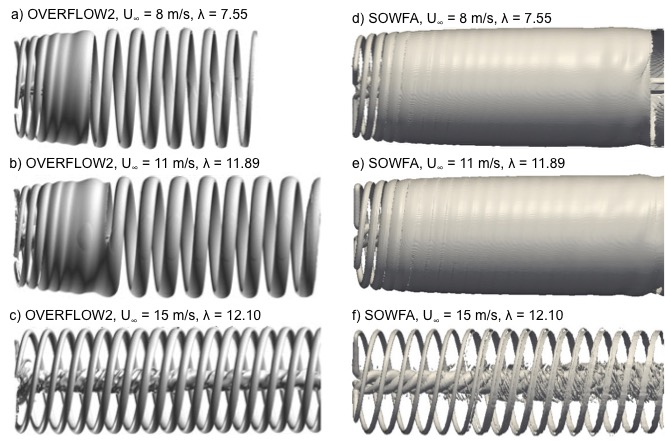
\includegraphics[width=\textwidth]{Figures/ch5Figures/isoVorts}
 \caption{ Iso-vorticity surfaces of the NREL 5-MW wake system for OVERFLOW2 and SOWFA simulations (Freestream flows from left to right. Images a,b, and c provided by R. Chow).}
 \label{isoVort}
\end{figure}   

\begin{figure}[htbp]
\centering
 \includegraphics[width=0.75\textwidth]{Figures/ch5Figures/VortMag}
 \caption{ Instantaneous vorticity magnitude at a center cut plane of the NREL 5-MW rotor at \emph{U$_\infty$} = 11 m/s using OVERFLOW2 (Freestream flows from left to right. Source: R. Chow). }
 \label{vortMag}
\end{figure}   

\begin{figure}[htbp]
\centering
 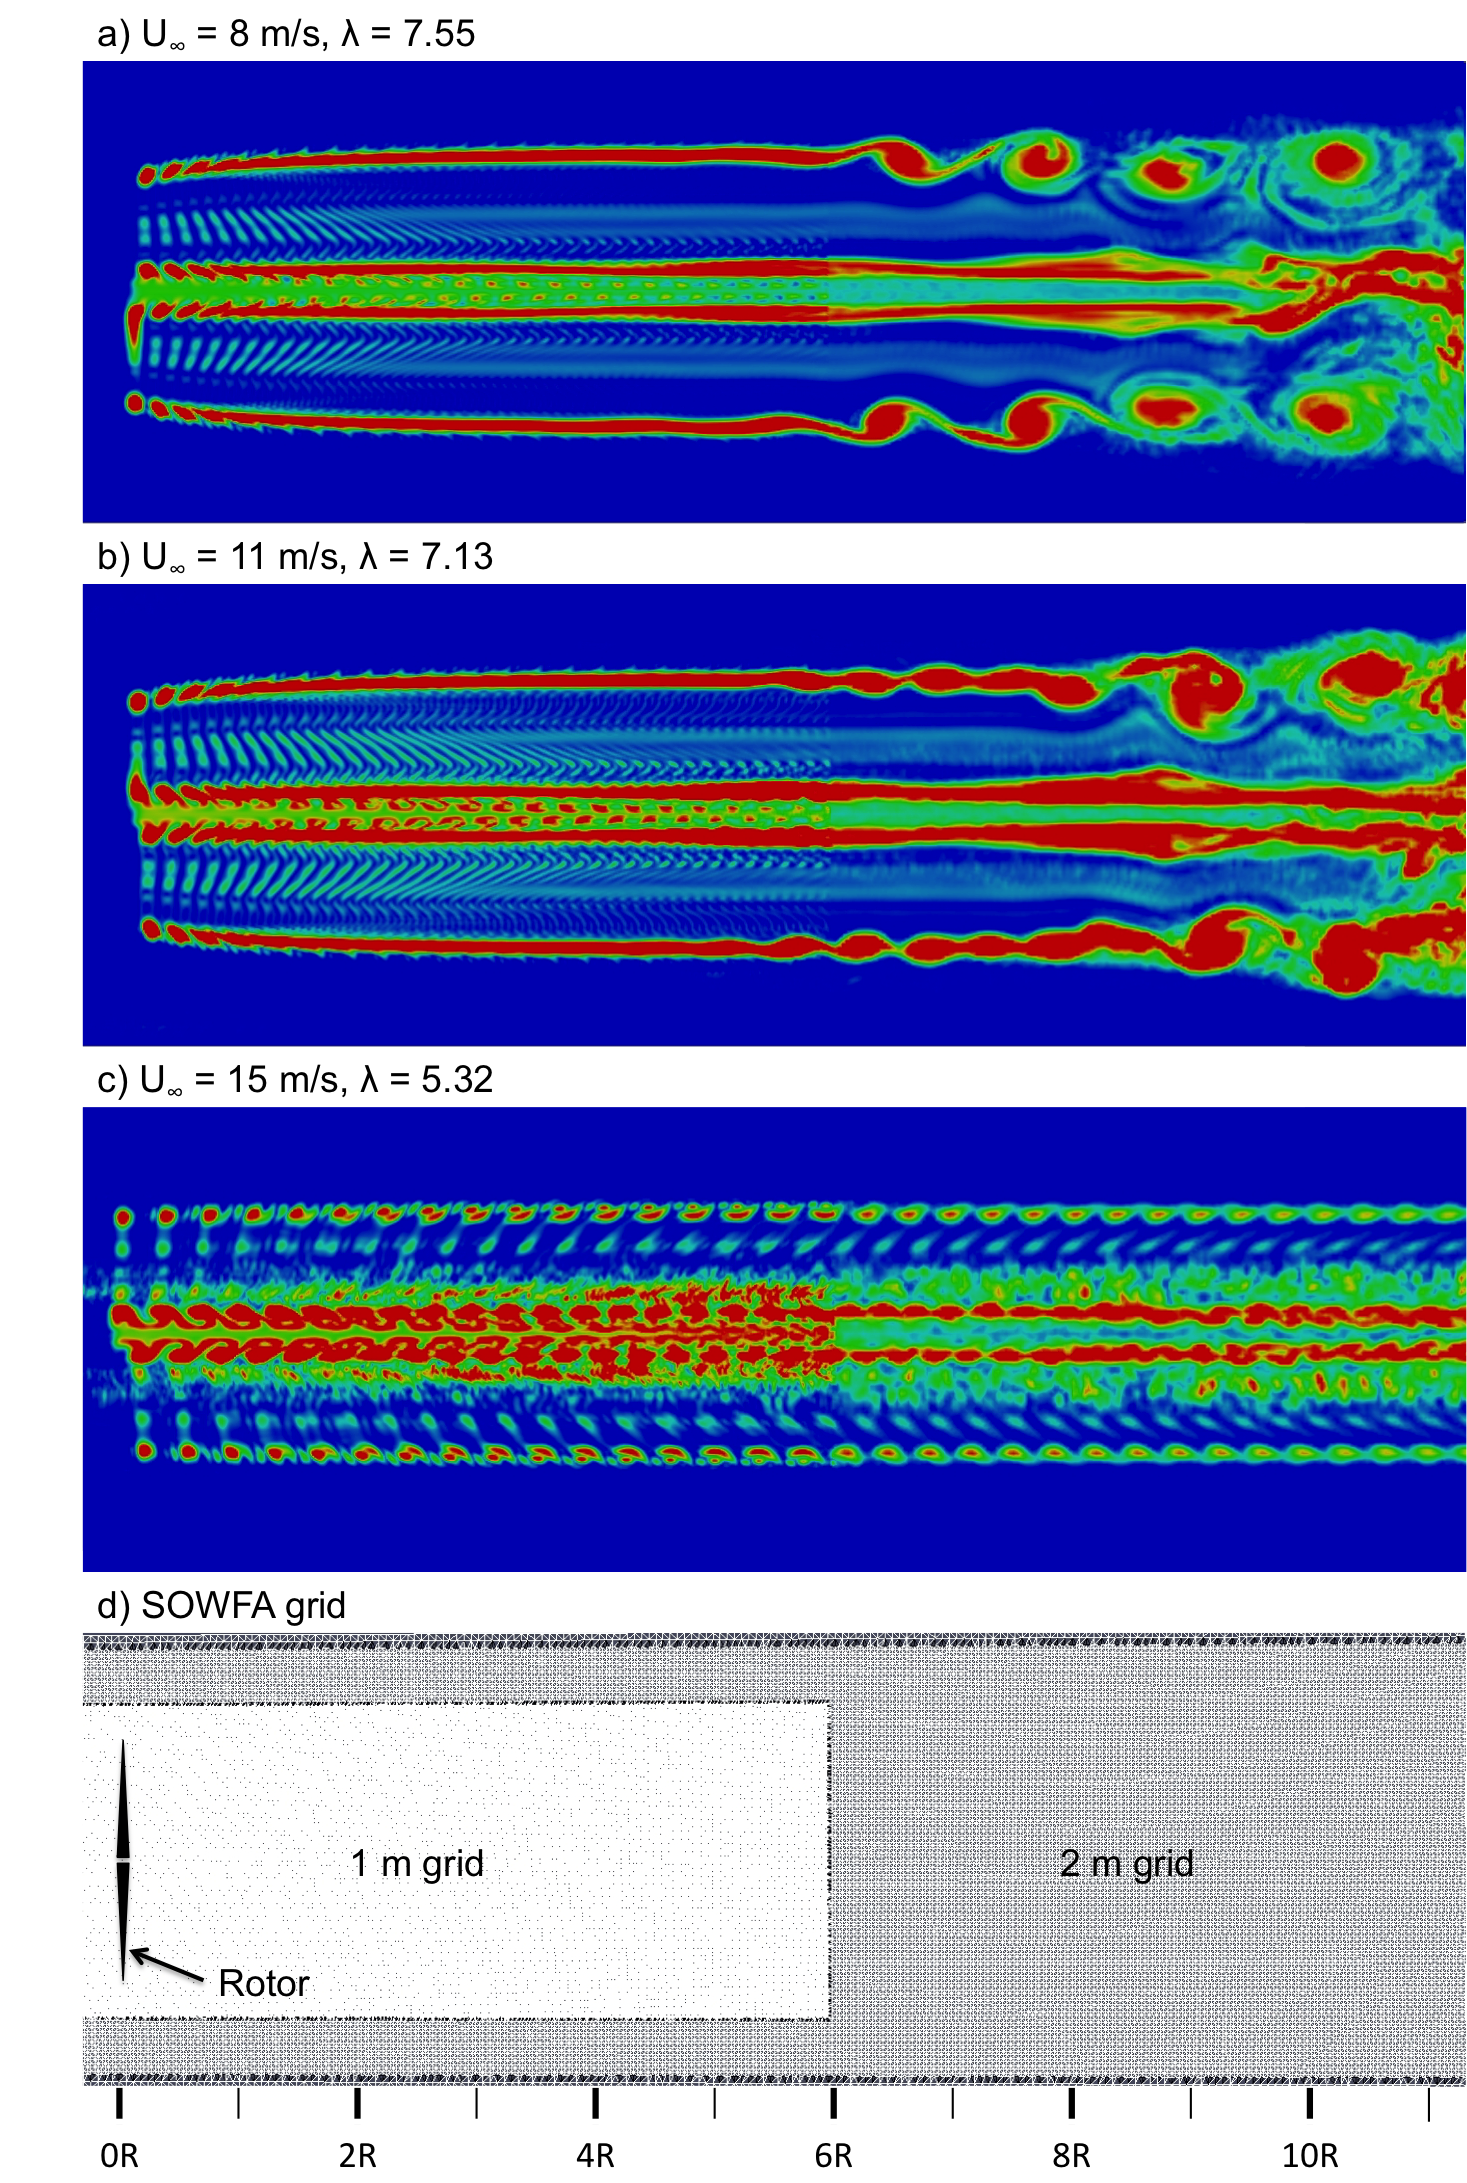
\includegraphics[width=0.85\textwidth]{Figures/ch5Figures/VortSlice_multSpeed}%
 \caption{ Instantaneous vorticity magnitude at a center cut plane of the NREL 5-MW rotor  for SOWFA simulations at \emph{U$_\infty$}=8, 11, and 15 m/s, as well as the SOWFA near-wake grid used in the simulations (Freestream flows from left to right).}
 \label{vortMag_multSpeed}
\end{figure}   




Figure \ref{fig5-5} shows the momentum deficit in the NREL 5-MW wake predicted by OVERFLOW2 and SOWFA for a range of stations downstream of the rotor. The downstream stations are at 10 m (0.16\emph{R}), 0.5\emph{R}, 1\emph{R}, 2\emph{R}, 4\emph{R}, 6\emph{R}, 8\emph{R}, and 12\emph{R}. A clear difference between the SOWFA and OVERFLOW2 results is the momentum deficit at the center of the rotor. For the first few downstream stations OVERFLOW2 predicts large momentum deficits in the blade root region whereas SOWFA predicts no momentum deficit. This discrepancy may be a contributing factor to the lower thrust values predicted by SOWFA, as seen in Table \ref{Table3}, and is likely caused by the difference in how SOWFA and OVERFLOW2 treat the rotor hub. OVERFLOW2 models the entire rotor, including the blades and a simplified version of the hub. SOWFA only models the blades, in effect modeling the rotor as if it had no hub. The \emph{U$_\infty$}=8, and 15 m/s cases also show significant discrepancies at the furthest downstream stations. At 8\emph{R} and 12\emph{R} downstream OVERFLOW2 shows the momentum deficit widening and decreasing in magnitude, especially near the edges of the wake. SOWFA results show the momentum deficit continuing to maintain its shape and magnitude. When the OVERFLOW2 results were originally generated the focus was on capturing power and thrust values sufficiently well\cite{chow2012}. Capturing the wake structure accurately was a necessary consequence and not the primary focus of the work. Because the far downstream wake behavior was of less interest in the original work and because of the high computational cost of these simulations, the far-wake grid used is coarser (8 - 16 m) than the SOWFA grid (2 m) at the 8\emph{R} and 12\emph{R} downstream stations. These downstream discrepancies occur when the coarser far-wake grids used in the OVEFLOW2 simulations can no longer support the fine structure details of the flow. Nevertheless there is good agreement between SOWFA and OVERFLOW2  with OVERFLOW2 generally showing slightly higher momentum deficits at the edges of the wake at most downstream stations. 

\begin{figure}[htbp]
 \centering
 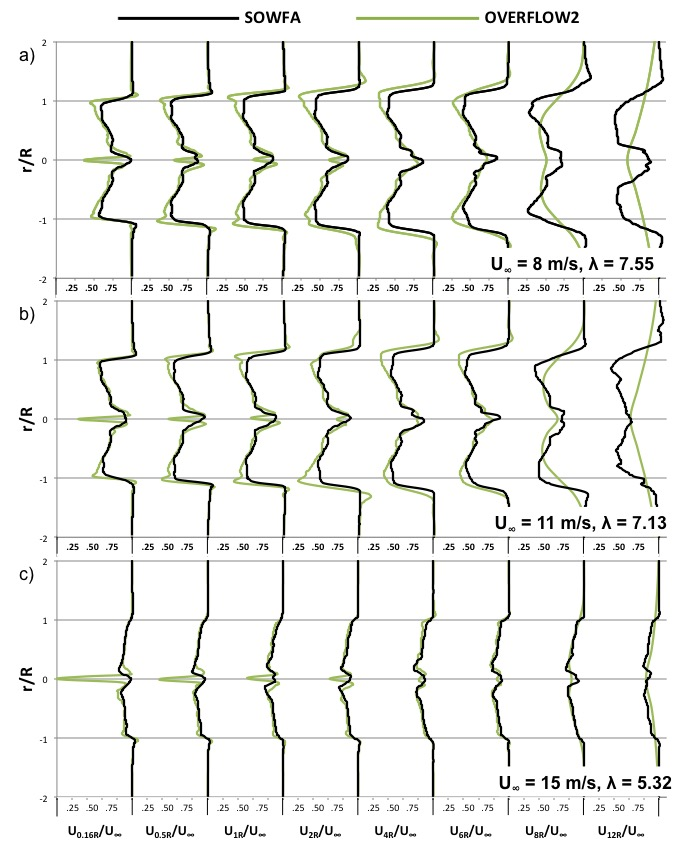
\includegraphics[width=0.75\textwidth]{Figures/ch5Figures/VelDef_SowfaOverflow}
 \caption{ Axial momentum deficit predicted by SOWFA and OVERFLOW2 for the NREL 5-MW rotor at \emph{U$_\infty$}=8, 11, and 15 m/s.}
 \label{fig5-5}
\end{figure}    





%-----------------------------------
%	SUBSECTION 4-2
%-----------------------------------

\subsection{Effects of Near-Wake Grid Length}\label{section5-4-2}
The size of the high resolution near-wake grid has a large effect on the number of grid cells in the simulation and therefore the amount of computing effort required to run a SOWFA simulation. In this section a study is carried out to examine how the downstream length of the near-wake affects rotor wake behavior. The purpose of this study is twofold, to gain insight into the grid length necessary to accurately capture wake behavior and to confirm that the SOWFA near-wake grid used for simulations in the previous section extends sufficiently far downstream. To examine the effect of near-wake grid length on wake behavior the \emph{U$_\infty$}=11 m/s SOWFA simulation case is modified by varying the downstream length of the near-wake grid. Simulations are carried out with near-wake grids extending 1\emph{R}, 2\emph{R}, and 12\emph{R} downstream. The results from these simulations are compared to each other as well as to results from the baseline \emph{U$_\infty$}=11 m/s simulation, which has a near-wake grid extending 6\emph{R} downstream. All other SOWFA simulation parameters remain unchanged except for a small change to the dimensions of the 2 m grid (Refinement Region \#4) for the 12\emph{R} simulation. In the 12\emph{R} simulation the downstream length of Refinement Region \#4 is extended from 12\emph{R} to 16\emph{R} to allow a smooth gradual transition between the 1 m near-wake grid and the 4 m grid.


The simulations produce identical thrust predictions and nearly identical power predictions, with the 1\emph{R} and 2\emph{R} cases producing slightly more power (5063 kW) than the 6\emph{R} and 12\emph{R} cases (5061 kW). Figure \ref{vortMag_Length} shows instantaneous vorticity magnitudes in cross sections of the wake. Though the wake behavior is similar for all four simulations, shorter near-rotor grids result in more loss of the detailed wake structure.  In the 1\emph{R} and 2\emph{R} cases some details of the wake tip vortex merging behavior is lost. The 1\emph{R} and 2\emph{R} cases also show the merged vortices breaking up into large vortical structures slightly sooner than the 6\emph{R} and 12\emph{R} cases. The wakes in the 6\emph{R} and 12\emph{R} cases show almost identical behavior until the vortical structures of the wakes break up and becomes chaotic approximately 10\emph{R} downstream.


Figure \ref{wakeDef_Length} shows the momentum deficit in the NREL 5-MW wake at a variety of stations downstream. Note that Figure \ref{wakeDef_Length} includes two additional downstream stations, 16\emph{R} and 20\emph{R}, that are not present in Figure \ref{fig5-5}. SOWFA is often used to study turbine to turbine wake interactions, where wake behavior more than 12\emph{R} downstream may be important. Therefore, the 16\emph{R} and 20\emph{R} stations were added to Figure \ref{wakeDef_Length} to capture wake behavior far downstream.  Up to 4\emph{R} downstream the momentum deficits are essentially identical for all simulations. At the 6\emph{R} and 8\emph{R} downstream stations the momentum deficit plots for the 1\emph{R} and 2\emph{R} simulation cases diverge slightly from the momentum deficit plots for the 6\emph{R} and 12\emph{R} simulation cases. The momentum deficits of the 1\emph{R} and 2\emph{R} simulation cases become slightly wider and show a slightly smaller maximum magnitude as the wake begins to break down. By the time the wakes reach  12\emph{R} downstream all four simulations are showing signs of the wake breaking down. The chaotic nature of the wakes at the 12\emph{R}, 16\emph{R}, and 20\emph{R} downstream stations causes the instantaneous momentum deficit plots to diverge for all four simulations.


\begin{figure}[htbp]
\centering
 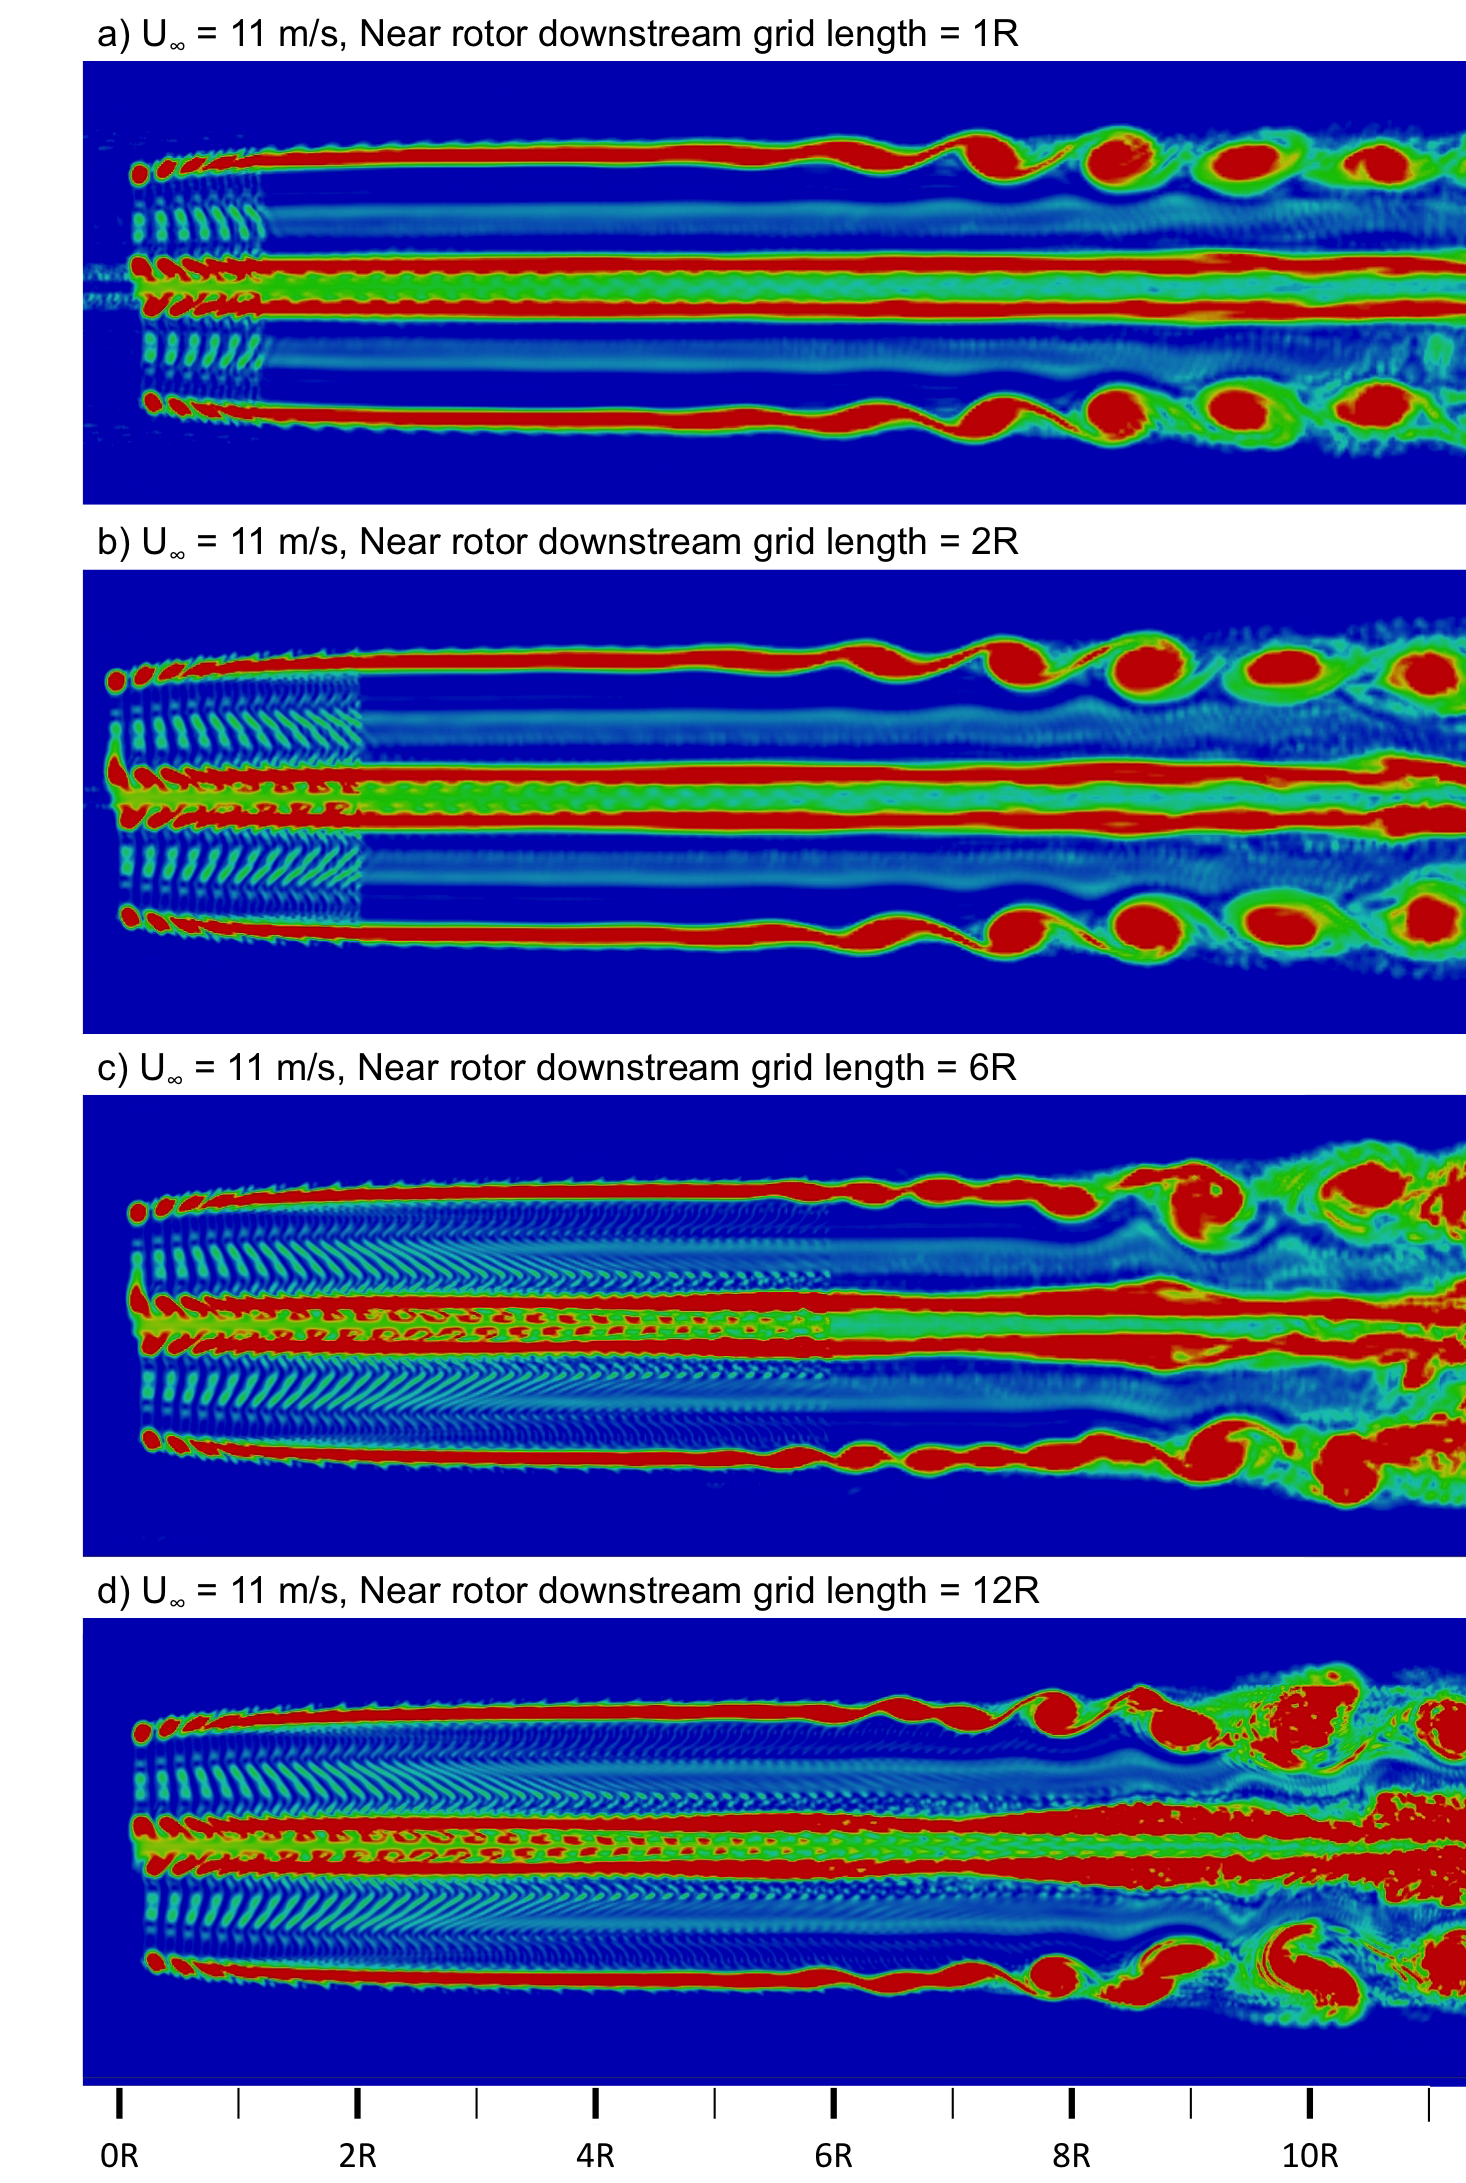
\includegraphics[width=0.85\textwidth]{Figures/ch5Figures/VortSlice_Length}%
 \caption{ Instantaneous vorticity magnitude at a center cut plane of the NREL 5-MW rotor  for SOWFA simulations at \emph{U$_\infty$}=11 m/s using near-wake grids of various lengths (Freestream flows from left to right). }
 \label{vortMag_Length}
\end{figure}   



\begin{figure}[htbp]
 \centering
 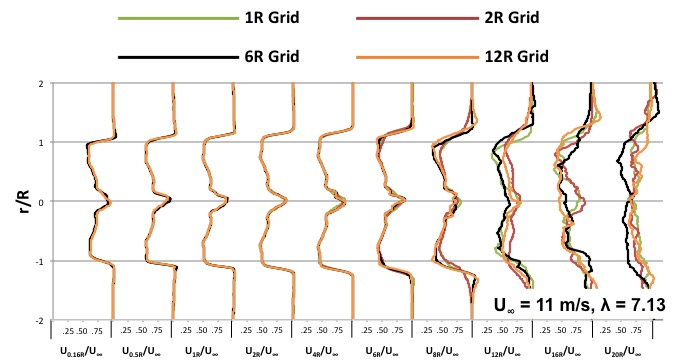
\includegraphics[width=0.75\textwidth]{Figures/ch5Figures/velDef_Length}
 \caption{ Axial momentum deficit predicted by SOWFA for NREL 5-MW rotor at \emph{U$_\infty$}=11 m/s using near-wake grids of various lengths. }

 \label{wakeDef_Length}
\end{figure}    



%-----------------------------------
%	SUBSECTION 4-3
%-----------------------------------

\subsection{Effects of Near-Wake Grid Resolution}\label{section5-4-3}
In previous sections we use a 1 m near-wake grid for SOWFA simulations. However, in practice SOWFA is often used with a coarser near-wake grid (~2.5-5 m)\cite{lee2012,fleming2014,archer2013,mache2014}. To examine the effect of near-wake grid resolution, SOWFA simulations of the \emph{U$_\infty$}=8, 11, and 15  m/s cases are run with a coarse near-wake grid and the results of those simulations are compared to the SOWFA simulation results in section  \ref{section5-4-1}. The coarse near-wake grid is generated by omitting two of the grid refinement steps described in section \ref{section5-2-4}. By not refining the grid in Refinement Regions \#4 and \#5, we get a near-wake grid that has the dimensions of Refinement Region \#3 (2.5\emph{R} upstream, 24.0\emph{R} downstream, 2.9\emph{R} radial) and is filled with 4 m $\times$ 4 m $\times$ 4 m cells.   Previous studies \cite{churchfield2012,martinez2012} have shown that the Gaussian projection width must be at least double the near-wake grid resolution for a stable solution. Therefore, the Gaussian projection width has been increased from the mean chord length of the NREL-5MW blade (3.5 m) to 8 m. All other SOWFA simulation parameters remain unchanged.

Table \ref{Table5} shows the power and thrust predicted by SOWFA when a 4 m near-wake grid is utilized as well as the percent diference between these results and the SOWFA results from section   \ref{section5-4-1}. The coarse grid causes an increase in the power and thrust predictions for all three cases.  Figure \ref{vortMag_resolution} shows instantaneous vorticity magnitudes in cross sections of the wake. By comparing Figure \ref{vortMag_resolution} to Figure \ref{vortMag_multSpeed} we can see how the use of a coarse 4 m near-wake grid affects wake behavior. Note that the images in Figure \ref{vortMag_resolution} extend 20\emph{R} downstream of the rotor, while the images in Figure \ref{vortMag_multSpeed} extend only 12\emph{R} downstream. The wakes in Figure \ref{vortMag_resolution} show far less detail than those shown in Figure \ref{vortMag_multSpeed}. Of particular interest, the strong tip vortices that can be seen forming and merging in Figures \ref{vortMag_multSpeed}a and \ref{vortMag_multSpeed}b are not present in Figures \ref{vortMag_resolution}a and \ref{vortMag_resolution}b. Figures \ref{vortMag_resolution}a and \ref{vortMag_resolution}b also show the wake extending much further downstream before breaking up, when compared to Figures \ref{vortMag_multSpeed}a and \ref{vortMag_multSpeed}b. The differences in wake behavior are less pronounced when we compare Figure \ref{vortMag_resolution}c to Figure \ref{vortMag_multSpeed}c. Though  Figure \ref{vortMag_resolution}c shows far less detail, the wake behavior does not seem to be fundamentally changed. Figure \ref{vortMag_resolution}c essentially looks like a lower resolution version of Figure \ref{vortMag_multSpeed}c.
 
\begin{table}
\centering
\begin{tabular}{c c c c c c c c c c}
\hline
 \emph{U$_{\infty}$}   & & {Power} &  {Thrust} & &  $\Delta$Power & $\Delta$Thrust\\
 (m/s) & & {(kW)} & {(kN)} & & {(\%)}  & {(\%)} \\
\hline
8   & & 2076 & 390 & & 4.6 & 2.1 \\
11 & & 5274 & 707 & & 4.2 & 2.0 \\
15 & & 5208 & 412 & & 2.2 & 1.7 \\
\hline
\end{tabular}
\caption{ Power and thrust predicted by coarse grid SOWFA simulations as well as the percent difference with fine grid simulations.}
\label{Table5}
\end{table}

\begin{figure}[htbp]
\centering
 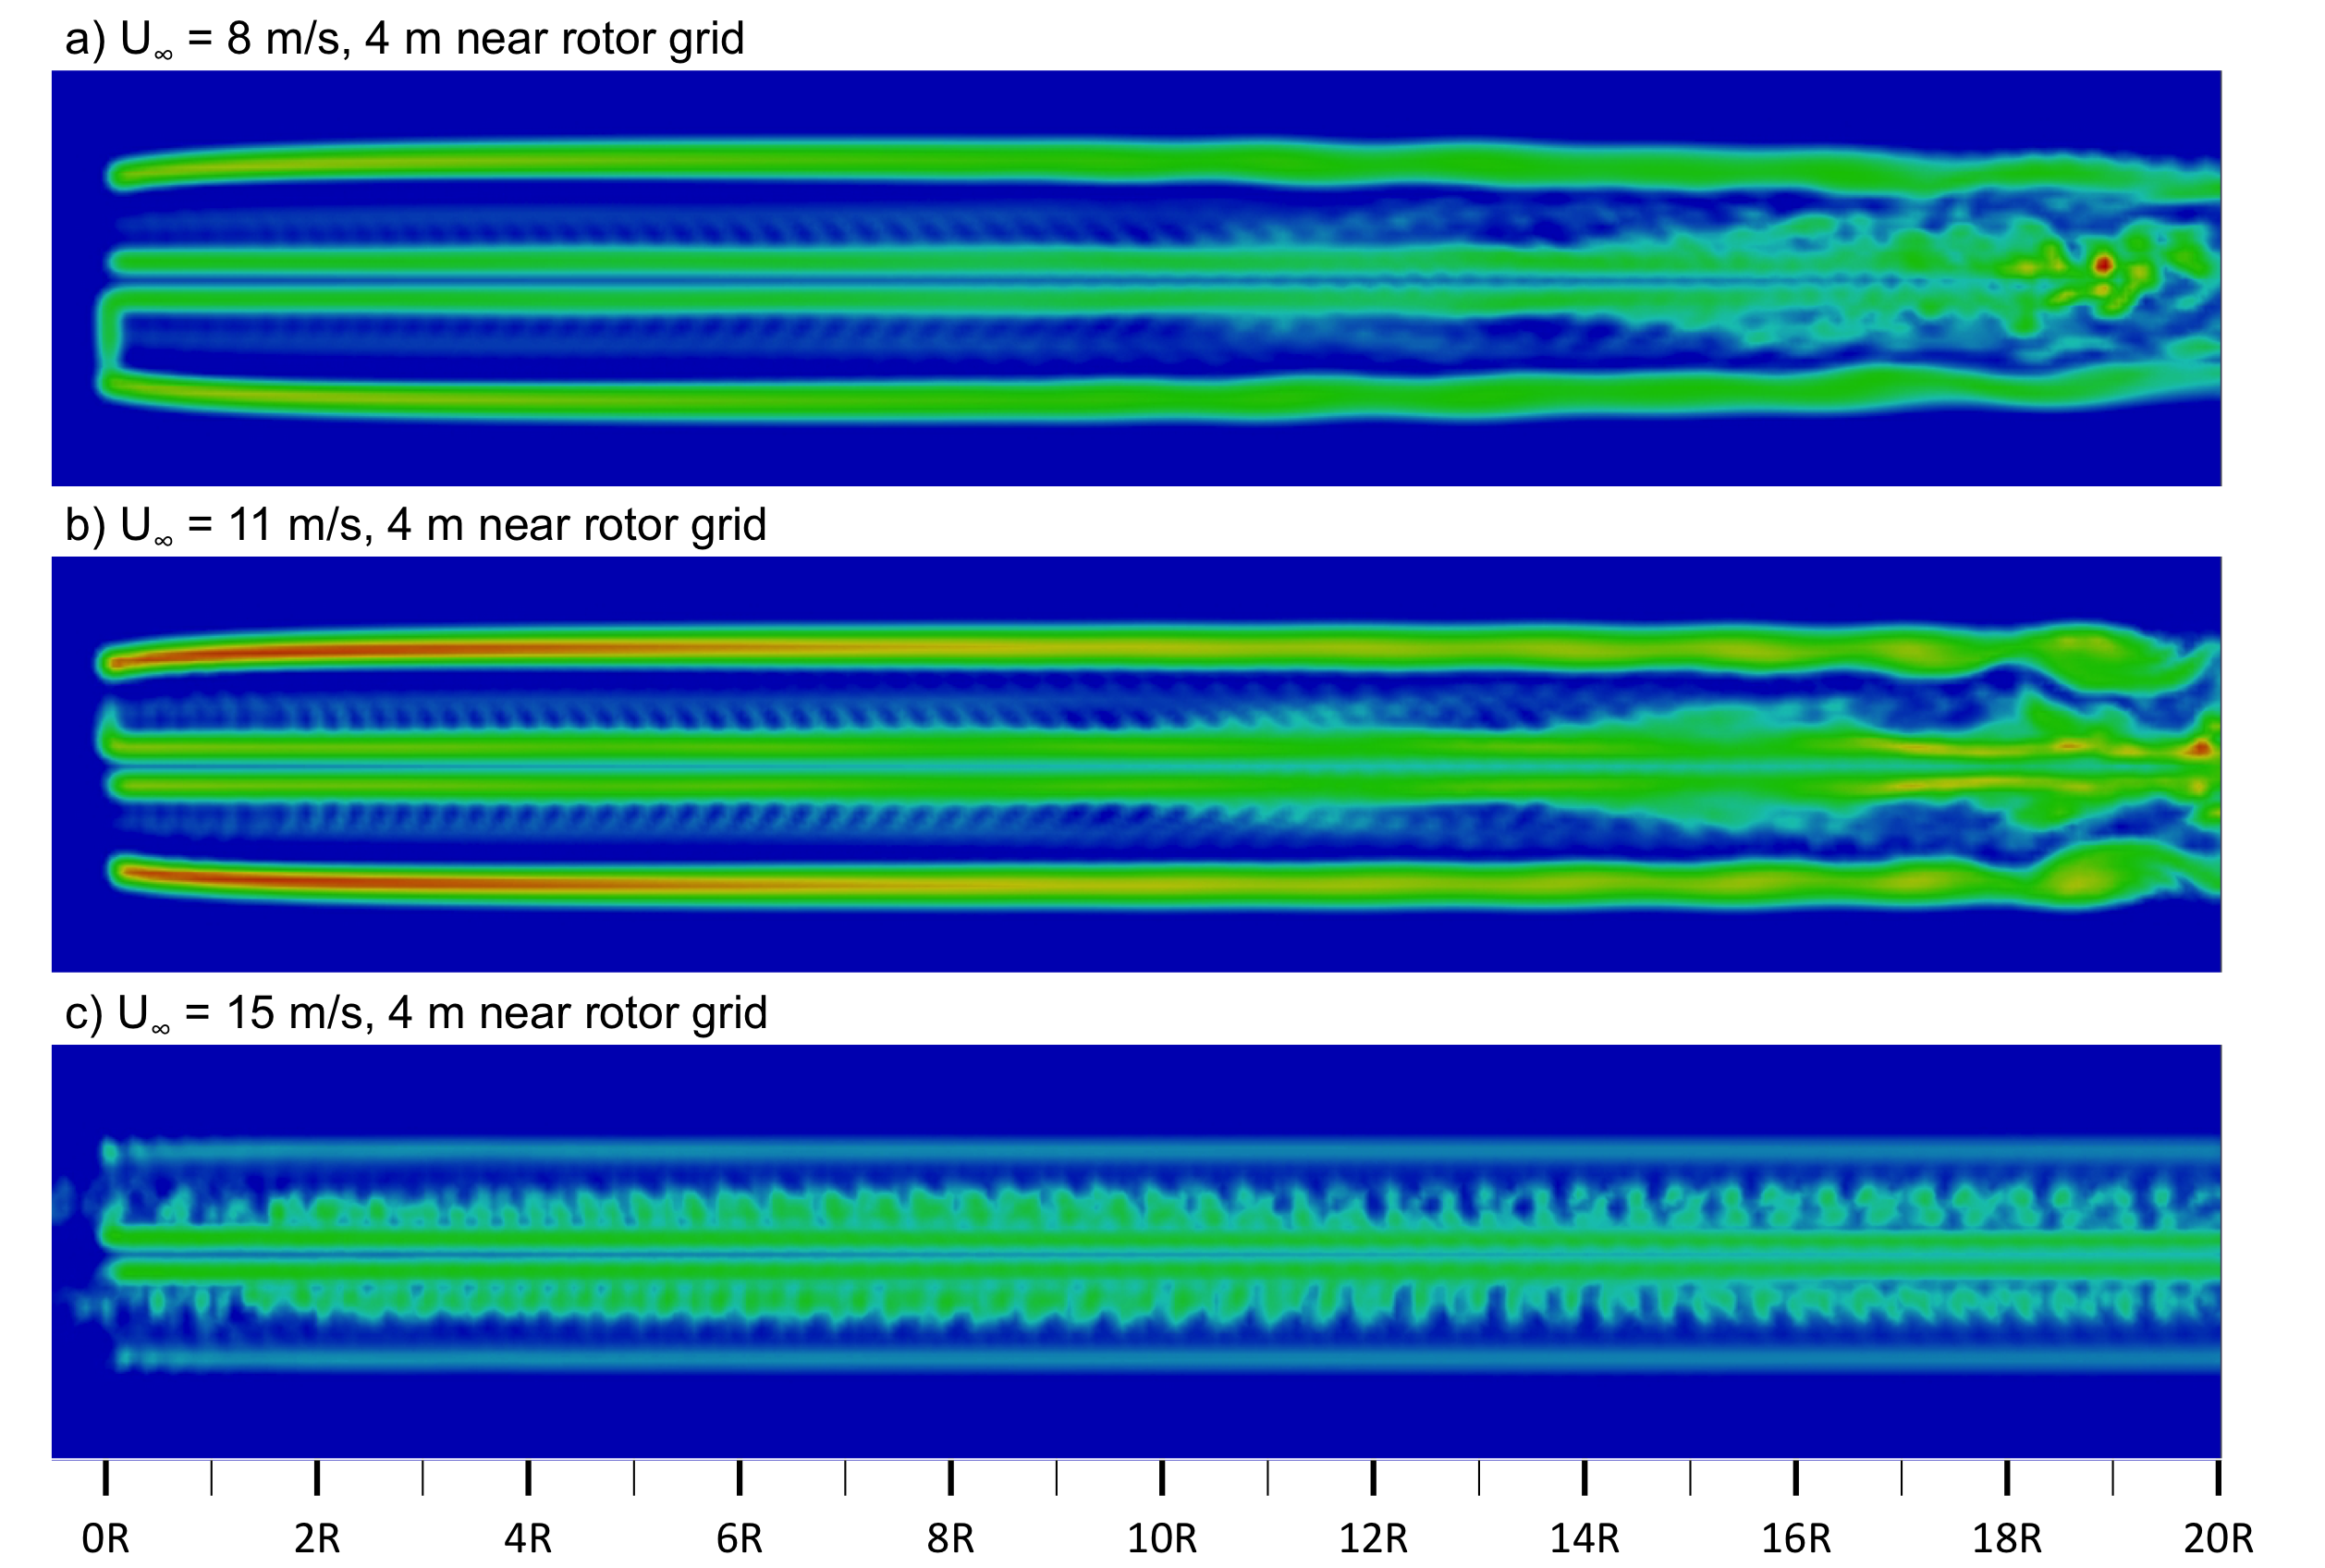
\includegraphics[width=.85\textwidth]{Figures/ch5Figures/VortSlice_Resolution}
 \caption{ Instantaneous vorticity magnitude at a center cut plane of the NREL 5-MW rotor  for SOWFA simulations at \emph{U$_\infty$}=8, 11, and 15 m/s, using a 4 m near-wake grid (Freestream flows from left to right). }
 \label{vortMag_resolution}
\end{figure}   


Figure \ref{wakeDef_resolution} shows the momentum deficit in the NREL 5-MW wake at a variety of stations downstream. The downstream stations shown are: 10 m (0.16\emph{R}), 0.5\emph{R}, 1\emph{R}, 2\emph{R}, 4\emph{R}, 6\emph{R}, 8\emph{R}, 12\emph{R}, 16\emph{R}, and 20\emph{R}.  At many of the downstream stations, the magnitude and shape of the momentum deficits predicted with the 4 m near-wake grid is similar to the magnitude and shape of the momentum deficit predicted with the 1 m near-wake grid. However, the momentum deficits in the coarse gird simulations show more gradual transitions near the center and edges of the wake, while the momentum deficits in the 1 m grid show sharper transitions. This makes sense based on the lower level of wake detail we see in Figure \ref{vortMag_resolution}. In figures \ref{wakeDef_resolution}a and \ref{wakeDef_resolution}b we see a larger discrepancy between the 1 m grid results and the 4 m grid results at the 16\emph{R} and 20\emph{R} downstream stations.  At those stations the 1 m grid results show the shape of the instantaneous momentum deficit becoming chaotic as the wake breaks down. The 4 m grid results show the momentum deficit retaining a smooth shape, while the width of the momentum deficit increases and the magnitude of the momentum deficit decreases. For the free stream velocity \emph{U$_\infty$}=8 m/s (Figure \ref{wakeDef_resolution}a) the 4 m grid results also show a larger momentum deficit magnitude than the 1 m grid results at the 16\emph{R} and 20\emph{R} downstream stations.


\begin{figure}[htbp]
 \centering
 \includegraphics[width=0.75\textwidth]{Figures/ch5Figures/VelDef_resolution}
 \caption{ Axial momentum deficit predicted by SOWFA for NREL 5-MW rotor at \emph{U$_\infty$}=8, 11, and 15 m/s, using both fine (1 m) and coarse (4 m) near-wake grids.}
 \label{wakeDef_resolution}
\end{figure}    





%----------------------------------------------------------------------------------------
%	SECTION 5
%----------------------------------------------------------------------------------------

\section{Conclusions}\label{section5-5}
The aerodynamic behavior predicted by OVERFLOW2 and SOWFA have been analyzed and compared for three laminar, steady, and uniform wind speed cases spread over the operating range of the NREL 5-MW turbine. Overall the results from OVERFLOW2 and SOWFA are found to have good agreement.  Power and thrust predictions are reasonably close, with SOWFA predicting higher power in \emph{U$_\infty$}=8 m/s and \emph{U$_\infty$}=11 m/s winds while predicting lower power in \emph{U$_\infty$}=15 m/s winds. SOWFA predicts slightly lower thrust for all three cases. In all cases the vortical structure of the wakes predicted by OVERFLOW2 and SOWFA were found to be very similar for the first 2\emph{R} downstream of the rotor. For the  \emph{U$_\infty$}=8 m/s and \emph{U$_\infty$}=11 m/s cases some differences between OVERFLOW2 and SOWFA were observed further downstream. The downstream momentum deficits predicted by the two simulation tools were found to have good agreement with a few exceptions. A discrepancy in momentum deficit near the center of the rotor can be explained by the difference in how OVERFLOW2 and SOWFA model the rotor hub. A discrepancy in the far downstream momentum deficits for the \emph{U$_\infty$}=8 m/s and \emph{U$_\infty$}=11 m/s  cases is consistent with the discrepancy seen in the far downstream wake behavior.

The effect of the downstream length of the near-wake grid has been examined. SOWFA simulations of an NREL 5-MW rotor in \emph{U$_\infty$}=11 m/s winds were conducted using near-wake grids of various lengths. The results show that extending the downstream length of the near-wake grid from 6\emph{R} to 12\emph{R} does not have an effect on wake behavior. This suggests that the 6\emph{R} long grid used for SOWFA simulations in section \ref{section5-4-1} is sufficiently long. Shortening the downstream length of the near-wake grid to 1\emph{R} or 2\emph{R} did have an effect on the wake behavior, but the effect was slight. In future simulations the small change in wake behavior caused by using a short near-wake grid may be a reasonable price to pay in order to reduce the grid size and computational cost of SOWFA simulations.

The effect of near-wake grid resolution was also examined. The \emph{U$_\infty$}=8 m/s, \emph{U$_\infty$}=11 m/s, and \emph{U$_\infty$}=15 m/s cases were simulated using near-wake SOWFA grids with 4 m resolution. The SOWFA results generated using a 4 m near-wake grid were then compared to the 1 m near-wake grid wake for SOWFA simulations in section \ref{section5-4-1}. Increasing the near-wake grid cell size to 4 m increased both the power and thrust predicted by SOWFA. The increased near-wake cell size also resulted in a significant loss of detailed wake behavior and some differences in the wake behavior far downstream. The differences were most prominent for the \emph{U$_\infty$}=8 m/s and \emph{U$_\infty$}=11 m/s cases, which lost the near-rotor tip vortex behavior seen in the 1 m grid results and showed the wake extending significantly farther downstream before breaking up. The momentum deficit predictions show good agreement, except for far downstream stations in the \emph{U$_\infty$}=8 m/s and \emph{U$_\infty$}=11 m/s cases.

Overall, the results documented in this chapter increase confidence in SOWFA and provide guidance for future SOWFA simulations. The results in Section \ref{section5-4-1} demonstrate that SOWFA can be tuned to have good agreement with more established wind turbine simulation tools like FAST and OVERFLOW2. Sections \ref{section5-4-2} and \ref{section5-4-3} provide insight into the effect of near rotor grid length and near rotor grid resolution. These insights will be valuable when designing future SOWFA simulations. In the following chapter, SOWFA will be used to simulate and evaluate the feed forward derating control scheme developed in Chapter \ref{Chapter4}. 